\documentclass{article}
\usepackage{a4wide}
\usepackage{graphicx}
\usepackage{caption}
\usepackage{amsmath}
\usepackage{subcaption}
\usepackage{fancyhdr}
\usepackage{physics}
\usepackage[utf8]{inputenc}
\usepackage[top=3cm, bottom=3cm, left=2cm, right=2cm]{geometry}

\author{Thomas Eboli}
\date{\today}
\title{Projet Introduction à l'imagerie numérique: Transfert de Style}

\begin{document}
\maketitle

\begin{abstract}
Ce projet porte sur la problématique de comprendre, implémenter et observer la technique de transfert de style d'une image (souvent un tableau) vers une photographie comme décrit dans \cite{DBLP:journals/corr/GatysEB15a}. Le code utilisé pour ces expériences est disponible à https://github.com/TheFeanor/Transfert-style.
\end{abstract}

\paragraph*{}La partie 1 portera sur l'écriture sous forme de problème d'optimisation du problème de transfert de style. La partie 2 portera sur l'intérêt des paramètres utilisés pour construire la fonction de perte à minimiser. La partie 3 portera sur les réponses du réseau de neurones à différents styles de peinture principalement.

\section{Modélisation sous forme d'un problème d'optimisation}
\paragraph*{}
Dans cette partie, je vais décrire le fonctionnement de la procédure utilisée pour générer des images par cette technique et son écriture sous forme d'un problème d'optimisation quadratique mais non-convexe.

\subsection*{Le réseau : le VGG-19}
\paragraph*{}
Le réseau utilisé est le fameux VGG-19 décrit dans \cite{DBLP:journals/corr/SimonyanZ14a}. Dans \cite{DBLP:journals/corr/MahendranV14}, les auteurs expliquent comment utiliser un tel réseau pour inverser des images à partir de chacune des couches. Leurs résultats ont montré que les premières couches retransmettent très bien l'image de départ car l'effet des non-linéarités n'est pas important voire nul pour conv1-1 et conv1-2. Plus on avance dans le réseau et plus les images deviennent "floues". Le réseau détruit l'image pour notre perception mais il apprend à reconnaître un paterne classique pour la catégorie figurant dans l'image ce qui est pratique pour faire de la classification faisant apparaître les idées de distance intra-classe et inter-classe.
 
\paragraph*{}
En pratique, le VGG-19 est utilisé principalement avec des couches de max pooling mais dans notre cas, les auteur de [1] préconisent d'utiliser des average pooling layers car les résultats sont meilleurs. Un comparatif des deux méthodes est détaillé dans la seconde partie.

\subsection*{La méthode}
\paragraph*{}
La méthode utilisée est un problème d'optimisation où il faut que l'on trouve une image $\hat x$ solution du problème d'optimisation :
\begin{equation}
min_x \alpha L_{contenu}(x, p) + \beta L_{style}(x, a)
\end{equation} 
\paragraph*{}
La variable $p$ désigne la photographie choisie et la variable $a$ l'image dont on veut extraire le style. Il est à noter que la fonction objectif est non-convexe et que le résultat est donc unique pour chaque itération. On tombe donc donc un minimum local de la fonction mais ce n'est pas grave car le problème est celui de la génération d'image; ça nous arrange même d'avoir quelque chose de nouveau à chaque fois à vrai dire !\\
On optimise par descente de gradient cette fonction objectif pour trouver la solution $\hat x$.

\subsubsection*{Perte liée au contenu}
\paragraph*{}
Le terme qui prend en compte le contenu de la fonction se calcule par la forme :
\begin{equation}
L_{contenu}(x,p) = \frac{1}{2} \sum_{i,j}(F_{i,j}^k-P_{i,j}^k)^2
\end{equation}
\paragraph*{}
Où, si on note $N_k$ le nombre de filtres pour la couche $k$ et $M_k$ le produit hauteur $\times$ d'un de ces filtres, alors $F_{i,j}^k$ est l'activation du $i$-ème filtre à la position $j$ dans la forme vectorisée des filtres pour la couche $k$ et pour l'image recherchée $x$. $P_{i,j}^k$ est la même activation mais pour la photo $p$.\\
Pour l'algorithme de rétro-propagation du gradient, on a besoin du gradient de cette perte. On obtient alors le gradient de cette perte par la formule :
\begin{equation}
\pdv{L_{contenu}}{F_{i,j}^k} = (F^k-P^k)_{i,j} \times ind_{F_{i,j}^k > 0}
\end{equation}
 
\subsubsection*{Perte liée au style}
\paragraph*{}
La perte liée au style est plus compliquée à calculer mais rien de bien horrible non plus. Contrairement à la perte liée au terme de structure et en accord avec les observations sur l'effet du VGG-19 à chaque couche, on prend l'information sur le style sur les couches conv1-1, conv2-1, conv3-1, conv4-1 et conv5-1. Chaque couche possède un niveau d'abstraction différent et donc une information différente sur le style de l'image. On considère d'abord les matrices de Gram qui mesurent les corrélations entre les divers canaux (on considère les versions vectorisées des activations !):
\begin{equation}
G_{i,j}^k = \sum_n F_{i,n}^k F_{j,n}^k
\end{equation}
\paragraph*{}
Si on note $G_{i,j}^k$ la matrice de corrélation associées aux activations des canaux $i$ et $j$ pour la couche $k$ et l'image à chercher $x$ et $A_{i,j}^k$ l'équivalent pour l'image dont on extrait le style, alors l'erreur pour la couche $k$ s'écrit:
\begin{equation}
E^k = \frac{1}{4 N_k^2 M_k^2} \sum_{i,j}(G_{i,j}^k-A_{i,j}^k)^2
\end{equation}
\paragraph*{}
On pondère chacune de ces pertes avec les poids $w_k$.  La perte totale s'écrit :
\begin{equation}
L_{style}(x, a) = \sum_k w_k E^k
\end{equation}
\paragraph*{}
Comme pour l'erreur sur le contenu, on cherche à rétro-propager l'erreur sur le style. Le gradient s'écrit:
\begin{equation}
\pdv{L_{style}}{F_{i,j}^k} = \frac{1}{N_k^2 M_k^2}(F^k)^T(G^k-A^k)_{i,j} \times ind_{F_{i,j}^k > 0}
\end{equation}

\section{Jouons avec les divers paramètres}
\paragraph*{}
On a tous les outils pour maintenant effectuer l'opération de transfert de style. Dans toute la suite, si on ne précise pas un paramètre, c'est qu'il prend sa valeur par défaut qui sont les suivantes :
\begin{enumerate}
\item poids $w_k = 0.2$  $\forall k$
\item couche de contenu : conv4-2
\item nombre d'itération $N = 500$
\item $\alpha = 1$, $\beta = 10^4$
\item pooling : average
\end{enumerate}

\paragraph*{}
Pour les mesures, j'utilise les images suivantes:
\begin{figure}[!htb]
\centering
\begin{minipage}{0.5\textwidth}
\centering
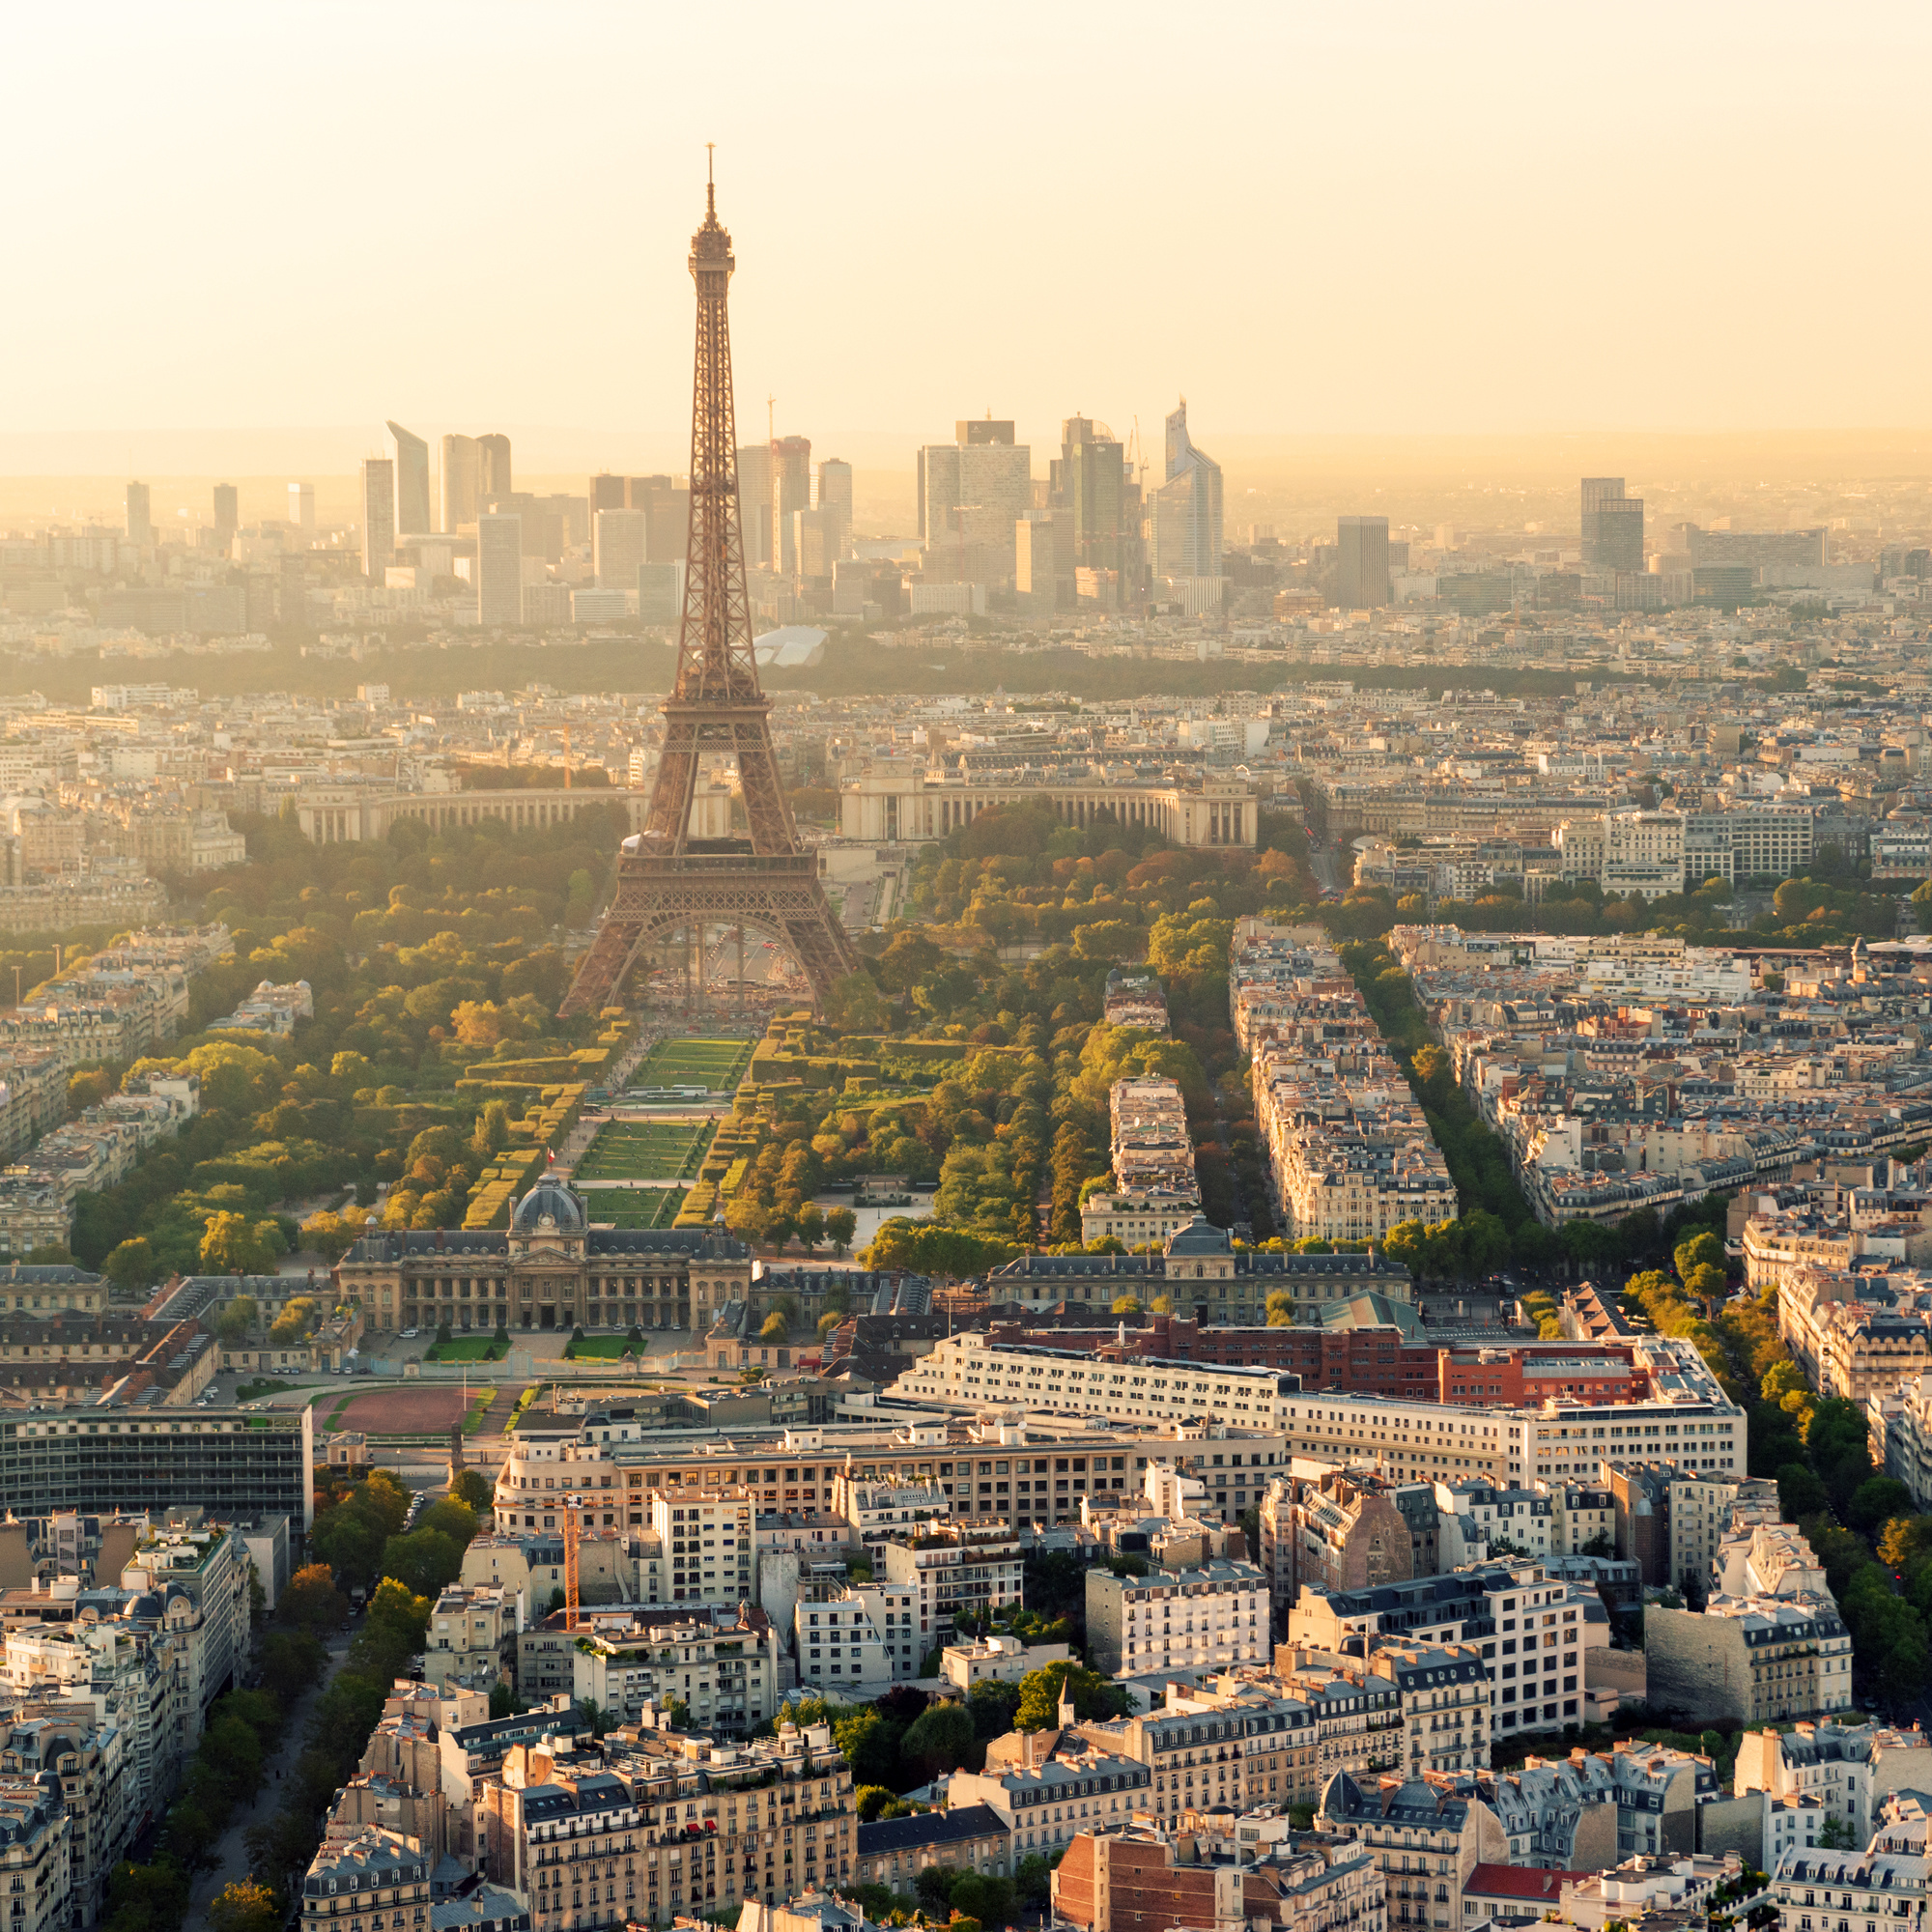
\includegraphics[width=0.77\textwidth]{../Images/paris.jpg}
\end{minipage}%
\begin{minipage}{0.5\textwidth}
\centering
\includegraphics[width=0.98\textwidth]{../Images/starry_night.jpg}
\end{minipage}
\label{fig:paris_starrynight}
\caption{\textit{Droite: $p$, Vue de Paris - Gauche: $a$, "Nuit étoilée" de Van Gogh}}
\end{figure}

\subsection*{Faire varier les couches de style}
\paragraph*{}
Je décide ici de faire varier les poids associés aux différentes couches servant à la représentation en terme de style de l'image à trouver $x$ et de l'image dont on extrait le style $a$.
\subparagraph*{Ne choisir qu'une couche}
J'ai essayé d'obtenir des images avec une seule couche de style mais la phase d'optimisation n’aboutit jamais car le gradient tombe très vite dans un minimum local. On ne peut donc tirer un quelconque résultat pertinent de cette partie.

\subparagraph*{Donner plus d'importance à certaines couches}
J'essaie avec des poids reflétant divers configurations où on donne plus de poids aux premières couches puis aux dernières couches.
J'utilise tour à tour les poids :
\begin{enumerate}
\item $w_1 = 0.6$, $w_2 = 0.1$, $w_3 = 0.1$, $w_4 = 0.1$, $w_5 = 0.1$
\item $w_1 = 0.35$, $w_2 = 0.25$, $w_3 = 0.2$, $w_4 = 0.15$, $w_5 = 0.05$
\item $w_1 = 0.1$, $w_2 = 0.1$, $w_3 = 0.6$, $w_4 = 0.1$, $w_5 = 0.1$
\item $w_1 = 0.05$, $w_2 = 0.15$, $w_3 = 0.2$, $w_4 = 0.25$, $w_5 = 0.35$
\item $w_1 = 0.1$, $w_2 = 0.1$, $w_3 = 0.1$, $w_4 = 0.1$, $w_5 = 0.6$
\end{enumerate}
\begin{figure}[!htb]
\centering
\begin{minipage}{0.2\textwidth}
\centering
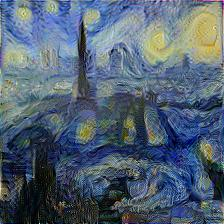
\includegraphics[width=0.98\textwidth]{../Images/transfer/paris_starrynight_w_06_01_01_01_01.jpg}
\end{minipage}%
\begin{minipage}{0.2\textwidth}
\centering
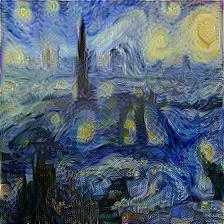
\includegraphics[width=0.98\textwidth]{../Images/transfer/paris_starrynight_w_035_025_02_015_005.jpg}
\end{minipage}%
\begin{minipage}{0.2\textwidth}
\centering
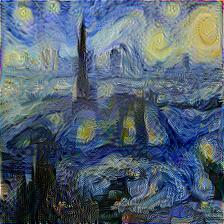
\includegraphics[width=0.98\textwidth]{../Images/transfer/paris_starrynight_w_01_01_06_01_01.jpg}
\end{minipage}%
\begin{minipage}{0.2\textwidth}
\centering
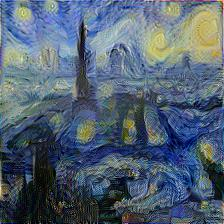
\includegraphics[width=0.98\textwidth]{../Images/transfer/paris_starrynight_w_005_015_02_025_035.jpg}
\end{minipage}%
\begin{minipage}{0.2\textwidth}
\centering
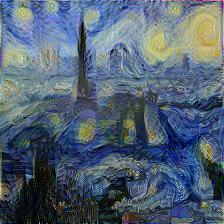
\includegraphics[width=0.98\textwidth]{../Images/transfer/paris_starrynight_w_01_01_01_01_06.jpg}
\end{minipage}
\label{fig:varier_poids}
\caption{\textit{Divers essais pour les configurations allant de 1 à 5 de gauche à droite}}
\end{figure}

On remarque que globalement modifier les poids n'amène pas à de grands changements mais lorsqu'on regarde de plus près, on peut apercevoir des étoiles en plus ou en mois suivant les configurations (par exemple au sommet de la tour Eiffel). Les immeubles de la Défense ou en premier plan sont légèrement différents d'une image à l'autre aussi (il vaut mieux regarder ces images sur un écran plutôt que sur une version imprimée). Chaque couche possède donc sa spécialité en quelques sortes même si globalement, le résultat possède un rendu identique dans chaque cas.

\subsection*{Faire varier la couche de contenu}
\paragraph*{}
Je fais varier les couches de style en choisissant tour à tour conv1-2, conv2-2, conv3-2, conv4-2 et conv5-2. La figure \ref{fig:varier_couche_contenu} expose les résultats obtenus.
\begin{figure}[!htb]
\centering
\begin{minipage}{0.2\textwidth}
\centering
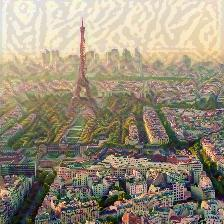
\includegraphics[width=0.98\textwidth]{../Images/transfer/paris_starrynight_c_conv_1_2.jpg}
\end{minipage}%
\begin{minipage}{0.2\textwidth}
\centering
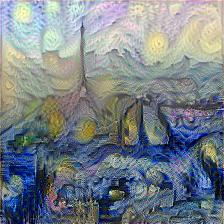
\includegraphics[width=0.98\textwidth]{../Images/transfer/paris_starrynight_c_conv_2_2.jpg}
\end{minipage}%
\begin{minipage}{0.2\textwidth}
\centering
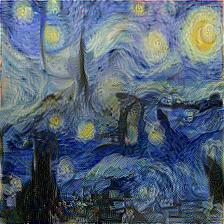
\includegraphics[width=0.98\textwidth]{../Images/transfer/paris_starrynight_c_conv_3_2.jpg}
\end{minipage}%
\begin{minipage}{0.2\textwidth}
\centering
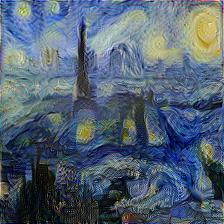
\includegraphics[width=0.98\textwidth]{../Images/transfer/paris_starrynight_1e4_500.jpg}
\end{minipage}%
\begin{minipage}{0.2\textwidth}
\centering
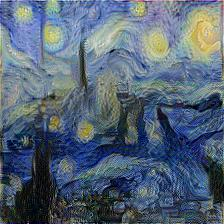
\includegraphics[width=0.98\textwidth]{../Images/transfer/paris_starrynight_c_conv_5_2.jpg}
\end{minipage}
\caption{\textit{De gauche à droite, des images allant de conv1-2 à conv5-2 pour le choix de la couche de structure}}
\label{fig:varier_couche_contenu}
\end{figure}

Pour des choix de couches de style basses comme conv1-2 et conv2-2, la méthode de descente de gradient mise en place n'aboutit pas et on obtient seulement des débuts de procédure de transfert de style. Pour conv1-2 on peut quand même voir que l'image commence à tourner autour des points définis comme des emplacements de soleild et les rues symétriques commencent à se tordre. Pour conv2-2, l'algorithme du gradient va plus loin et on voit apparaître plus nettement l'effet du transfert mais on conserve encore très nettement le style de la photographie de Paris. Pour les essais sur les couches suivantes, les non-linéarités du réseau commencent à se faire sentir. On commence à franchement perdre la structure au profit du style. L'algorithme converge enfin. Plus on choisit une couche élevée pour le la structure et plus l'image se met à tourner, plus on perd le détail des immeubles et même de la tour Eiffel. Il est amusant de noter que l'avenue menant au Champs de Mars est comprise comme un immeuble et la tour visible sur "Nuit Étoilée" est transposée sur cette avenue. Dans la dernière image, on ne conserve tellement plus d'information sur le contenu que la tour Eiffel est presque effacée !

\subsection*{Faire varier le nombre d'itérations}
\paragraph*{}
Je fais varier le nombre d'itérations $N$ en choisissant tour à tour 5, 50, 100, 250 et 500. Les résultats se trouvent dans la figure \ref{fig:varier_iteration}.
\begin{figure}[!htb]
\centering
\begin{minipage}{0.2\textwidth}
\centering
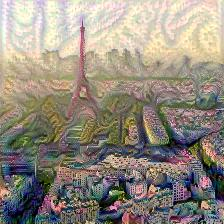
\includegraphics[width=0.98\textwidth]{../Images/transfer/paris_starrynight_1e4_5.jpg}
\end{minipage}%
\begin{minipage}{0.2\textwidth}
\centering
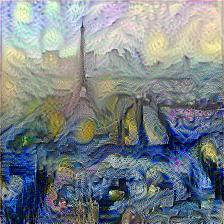
\includegraphics[width=0.98\textwidth]{../Images/transfer/paris_starrynight_1e4_50.jpg}
\end{minipage}%
\begin{minipage}{0.2\textwidth}
\centering
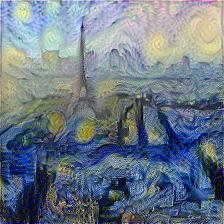
\includegraphics[width=0.98\textwidth]{../Images/transfer/paris_starrynight_1e4_100.jpg}
\end{minipage}%
\begin{minipage}{0.2\textwidth}
\centering
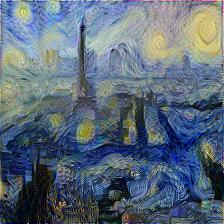
\includegraphics[width=0.98\textwidth]{../Images/transfer/paris_starrynight_1e4_250.jpg}
\end{minipage}%
\begin{minipage}{0.2\textwidth}
\centering
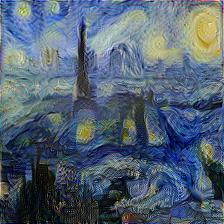
\includegraphics[width=0.98\textwidth]{../Images/transfer/paris_starrynight_1e4_500.jpg}
\end{minipage}
\caption{\textit{De gauche à droite, des images allant de 5 à 500 pour le choix de $N$}}
\label{fig:varier_iteration}
\end{figure}

Phénomène déjà visible dans la section précédent, le nombre d'itérations est primordial pour permettre un transfert efficace du style d'une image vers une autre. Ainsi Pour de petits nombres d'itérations, la photographie s'imprègne que très peu du style. On voit apparaître des formes psychédéliques dans le ciel puis petit à petit les étoiles et la couleur. Les bâtiments se tordent au fur et à mesure que les étapes se succèdent pour finalement produire un résultat probant autour de 500 itérations (convergence).

\subsection*{Faire varier $\alpha$ et $\beta$}
\paragraph*{}
Je touche ici au cœur du problème d'optimisation en modifiant aux poids $\alpha$ et $\beta$ et plus particulièrement à $\beta$ car optimiser $\alpha L_{contenu}+\beta L_{style}$ est équivalent à minimiser $L_{contenu}+ \frac{\beta}{\alpha} L_{style}$. Donc en fixant $\alpha=1$, je n'ai plus qu'à jouer sur $\beta$.\\
Je fais varier le ratio $\frac{\beta}{\alpha}$ en choisissant tour à tour $\beta =$ 1, 10, 100, 1000, 10000 et 100000. Les résultats sont visibles à la figure \ref{fig:varier_beta}
\begin{figure}[!htb]
\centering
\begin{minipage}{0.16\textwidth}
\centering
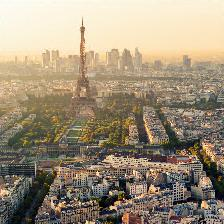
\includegraphics[width=0.98\textwidth]{../Images/transfer/paris_starrynight_1e0_500.jpg}
\end{minipage}%
\begin{minipage}{0.16\textwidth}
\centering
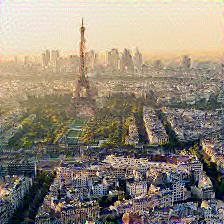
\includegraphics[width=0.98\textwidth]{../Images/transfer/paris_starrynight_1e1_500.jpg}
\end{minipage}%
\begin{minipage}{0.16\textwidth}
\centering
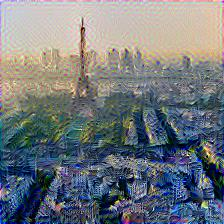
\includegraphics[width=0.98\textwidth]{../Images/transfer/paris_starrynight_1e2_500.jpg}
\end{minipage}%
\begin{minipage}{0.16\textwidth}
\centering
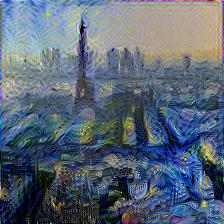
\includegraphics[width=0.98\textwidth]{../Images/transfer/paris_starrynight_1e3_500.jpg}
\end{minipage}%
\begin{minipage}{0.16\textwidth}
\centering
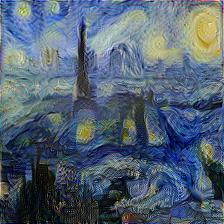
\includegraphics[width=0.98\textwidth]{../Images/transfer/paris_starrynight_1e4_500.jpg}
\end{minipage}%
\begin{minipage}{0.16\textwidth}
\centering
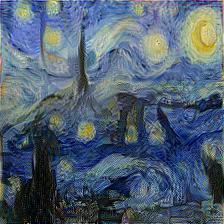
\includegraphics[width=0.98\textwidth]{../Images/transfer/paris_starrynight_1e5_500.jpg}
\end{minipage}
\caption{\textit{De gauche à droite, des images avec un choix de $\beta$ allant de 1 à 100000}}
\label{fig:varier_beta}
\end{figure}

On observe que pour des valeurs de $\beta$ relativement faibles et comparables à $\alpha$, le style n'est pas transféré ou très peu vers la photographie de Paris. Pour des valeurs plus fortes (à partir de 10000), l'opération se fait et pour la valeur maximale, on transfère tellement de style qu'on perd énormément de détails. Par exemple le quartier de la Défense est totalement noyé, les immeubles en premier plan aussi et la tour Eiffel disparaît à nouveau. Mettre beaucoup de style semble équivalent et ne pas considérer beaucoup de structure comme dans le cas du choix de conv5-2 pour la couche de structure. On retombe bien sur nos pieds.

\subsection*{Faire varier le type de pooling}
Dans \cite{DBLP:journals/corr/GatysEB15a}, les auteurs affirment qu'ils ont de meilleurs résultats avec un couche average pooling plutôt qu'avec les couches de max pooling classiques ou de stochastic pooling comme décrit dans \cite{DBLP:journals/corr/abs-1301-3557}. Ils ne fournissent pas d'illustrations de ce propos donc je propose de fournir un exemple pour avoir le coeur net à la figure \ref{fig:pooling_difference}.
\begin{figure}[!htb]
\centering
\begin{minipage}{0.33\textwidth}
\centering
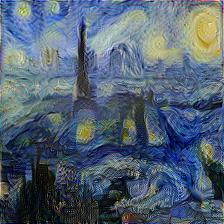
\includegraphics[width=0.75\textwidth]{../Images/transfer/paris_starrynight_1e4_500.jpg}
\end{minipage}%
\begin{minipage}{0.33\textwidth}
\centering
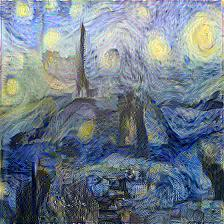
\includegraphics[width=0.75\textwidth]{../Images/transfer/paris_starrynight_MAX.jpg}
\end{minipage}%
\begin{minipage}{0.33\textwidth}
\centering
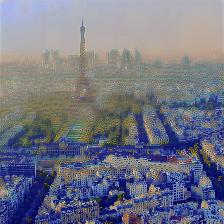
\includegraphics[width=0.75\textwidth]{../Images/transfer/paris_starrynight_STOCHASTIC.jpg}
\end{minipage}
\caption{A gauche, le average pooling, au milieu le max pooling et à droite le stochastic pooling}
\label{fig:pooling_difference}
\end{figure}

Les auteurs de \cite{DBLP:journals/corr/GatysEB15a} choisissent le average pooling car il permet de mieux rétro-propager le gradient et ça se voit ! Les deux autres techniques détruisent beaucoup d'informations à chaque étape en ne gardant que certains pixels de chaque patch alors que la méthode par moyenne conserve un peu d'information de chacun de pixels. Avec de petits filtres comme ceux du VGG-19, on peut même espérer en tombant sur des zones uniformes de reconstruire l'information très fidèlement car la moyenne de la zone uniforme est très proche de la valeur de chacun des pixels de cette zone.

\section{Jouons avec les styles artistiques}
\paragraph*{}
On a vu que la méthode de transfert de style fonctionnait bien avec les bons paramètres pour "Nuit Étoilée" de Van Gogh mais que se passe-t-il maintenant si on change le style du tableau ? Chaque mouvement en peinture se définit par le style que partagent les artistes d'une même périodes et certains sont plus fidèles à la réalité que d'autres et certaines œuvres font plus apparaître des lignes et des structures que d'autres (ce qui n'est pas le cas des œuvres de Van Gogh !). Un cas d'école est d'opposer Ingres et Delacroix, c'est la ligne contre la couleur.\\
Je propose donc d'exhiber ces différences en le faisant non pas sur un paysage mais une photographie de moi-même pour des raisons de droit à l'apparition et pour ne pas ressortir la sempiternelle image de Lenna, on l'a assez vue. Un visage possède plusieurs zones uniformes et pleins de détails donc on peut tester les capacités de la méthode sur plusieurs configurations de pixels. Pour ce qui est des tableaux, je pioche dans les paysages et les portraits pour voir si la structure du tableau influe un peu, beaucoup ou pas du tout dans la qualité du transfert. La photographie de départ est la figure \ref{fig:tdf} et les résultats sont les figures \ref{fig:set_1}, \ref{fig:set_2}, \ref{fig:set_3}, \ref{fig:set_4}, \ref{fig:set_5} et \ref{fig:set_6}.

\begin{figure}[!htb]
\centering
\begin{minipage}{0.5\textwidth}
\centering
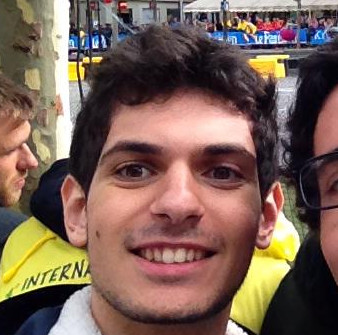
\includegraphics[scale=0.5]{../Images/tdf.jpg}
\caption{\textit{Une photo pendant l'arrivée du Tour de France à Paris}}
\label{fig:tdf}
\end{minipage}%
\begin{minipage}{0.5\textwidth}
\paragraph*{} J'ai choisi cette image pour les raisons mentionnées plus haut mais aussi car on peut apercevoir un visage au second plan et un arbre qui est une structure droite qui possède quelques détails puis en arrière-plan une foule et quelques structures complexes comme les stores. Il y a matière à voir différents effets sur cette image donc. 
\end{minipage}
\end{figure}

\begin{figure}[!htb]
\centering
\begin{minipage}{0.25\textwidth}
\centering
\includegraphics[width=0.98\textwidth]{../Images//starry_night.jpg}
\end{minipage}%
\begin{minipage}{0.25\textwidth}
\centering
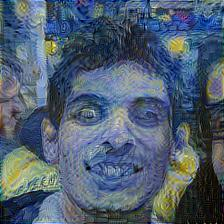
\includegraphics[width=0.98\textwidth]{../Images/transfer/tdf_starrynight.jpg}
\end{minipage}%
\begin{minipage}{0.25\textwidth}
\centering
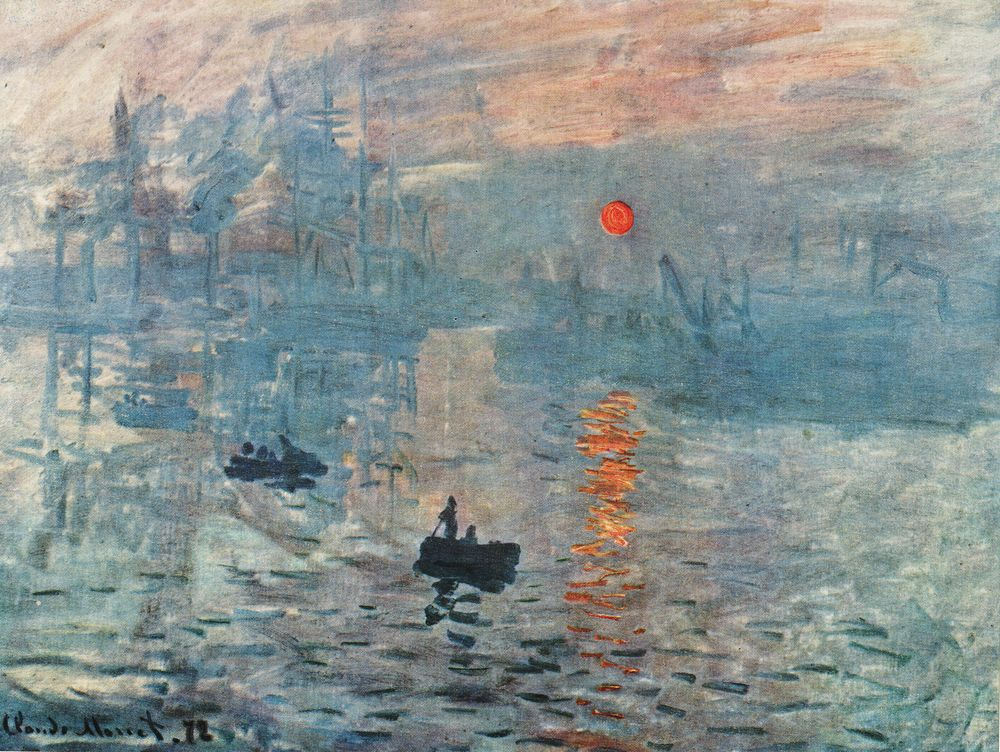
\includegraphics[width=0.98\textwidth]{../Images/Impression_soleil_levant_r.jpg}
\end{minipage}%
\begin{minipage}{0.25\textwidth}
\centering
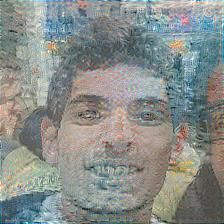
\includegraphics[width=0.98\textwidth]{../Images/transfer/tdf_impression.jpg}
\end{minipage}
\caption{\textit{Gauche: Nuit étoilée de Van Gogh - Droite: Impression Soleil Levant de Monet}}
\label{fig:set_1}
\end{figure}

\paragraph*{Nuit Étoilée - fig \ref{fig:set_1}} Les structures sont respectées et là où il y a du jaune dans l'image initiale il y a des étoiles. Le visage étant une zone uniforme, un même ton est utilisé (celui de l'espèce de nuage semble-t-il). Le second visage possède une couleur plus proche de la chair montrant que le réseau considère le visage du badaud et le mien comme deux choses différents. La présence d'un arbre puis d'un fond est elle aussi respectée car une étoile est estompée par le tronc. L'aspect des maisons se retrouve dans la modélisation de la foule au fond ainsi que dans les yeux et les dents. qui sont des zones particulières qui tranchent avec l'uniformité de la peau.

\paragraph*{Impression Soleil Levant - fig \ref{fig:set_1}} Comme précédemment, ce qui frappe, c'est que l'algorithme cherche à associer des zones de même couleurs. La chair est proche de la couleur du ciel du tableau donc la peau ressemble au ciel avec quelques zones d'eau. Le rouge est modélisé par des ersatz de soleils et les cheveux prennent la couleur du port de Londres dans la brume. Le tableau ne possédant pas de structures comme les maisons dans l’œuvre précédente, les zones de détail comme la foule, les yeux et les dents sont moins bien rendus.

\begin{figure}[!htb]
\centering
\begin{minipage}{0.25\textwidth}
\centering
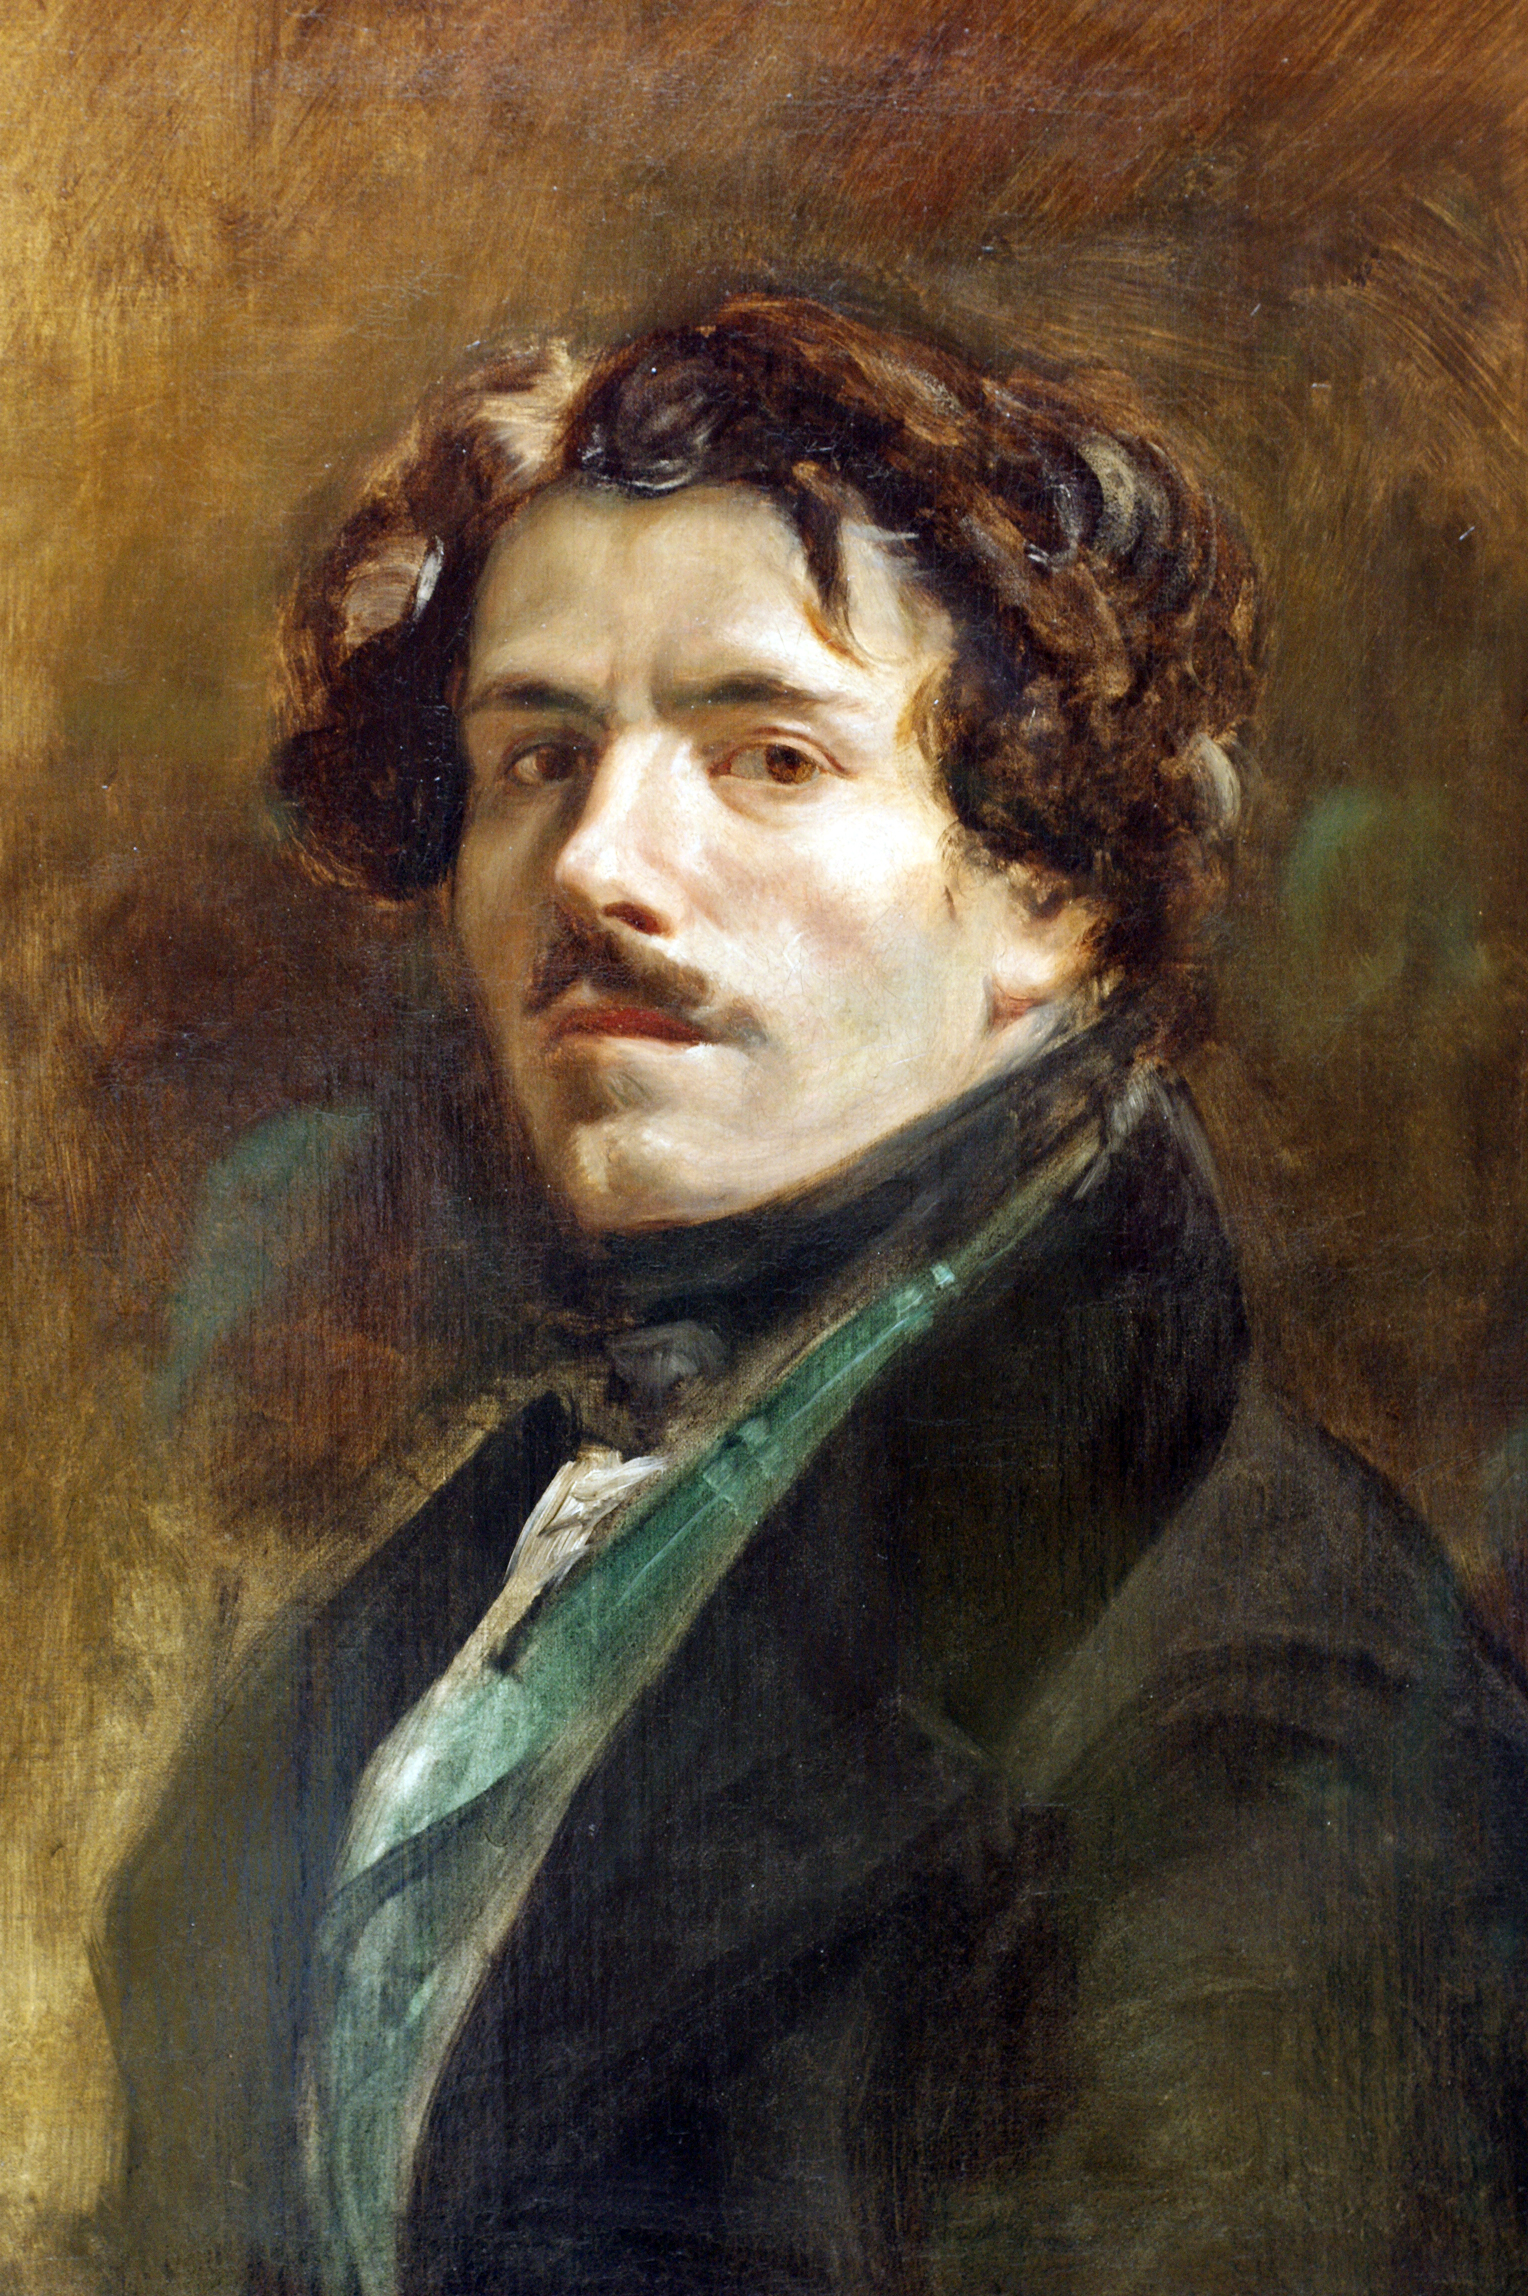
\includegraphics[width=0.98\textwidth]{../Images/delacroix.jpg}
\end{minipage}%
\begin{minipage}{0.25\textwidth}
\centering
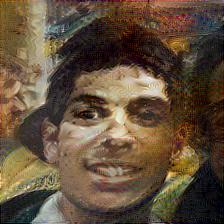
\includegraphics[width=0.98\textwidth]{../Images/transfer/tdf_delacroix.jpg}
\end{minipage}%
\begin{minipage}{0.25\textwidth}
\centering
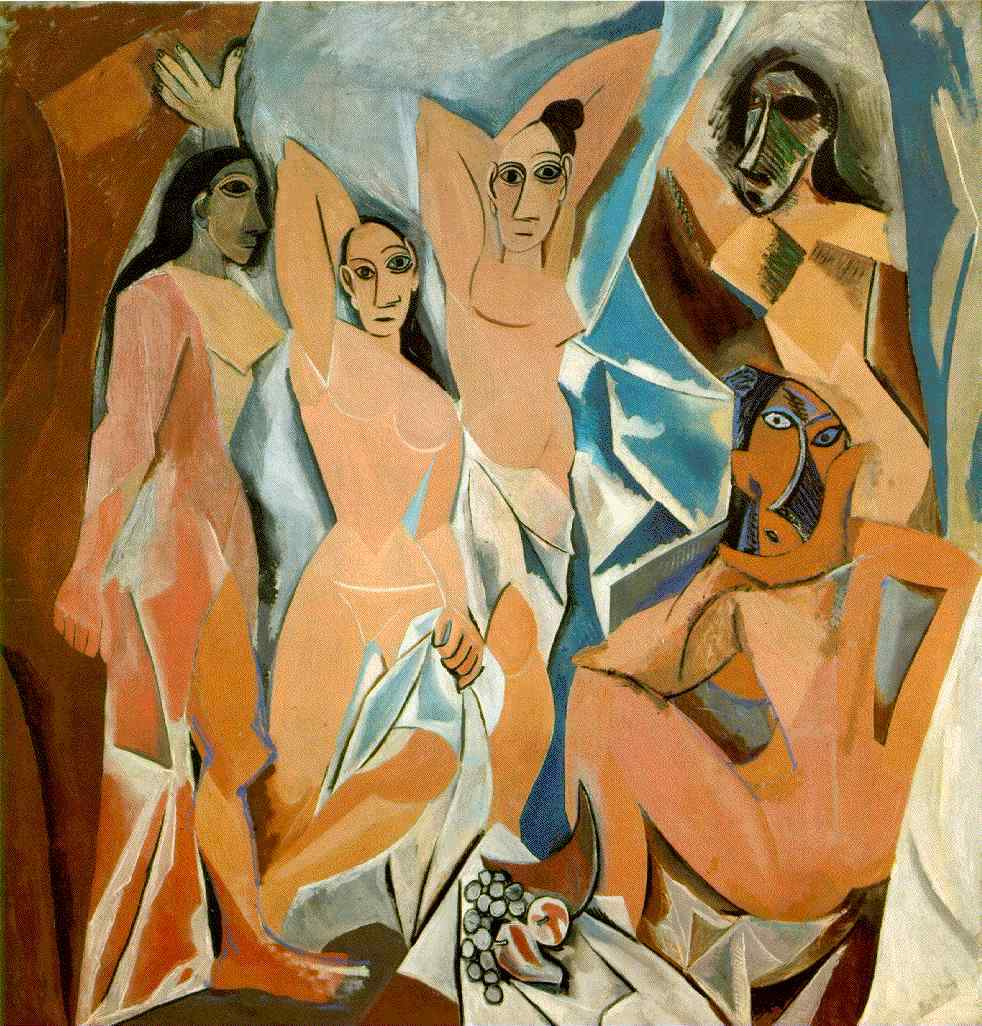
\includegraphics[width=0.98\textwidth]{../Images/demoiselles.jpg}
\end{minipage}%
\begin{minipage}{0.25\textwidth}
\centering
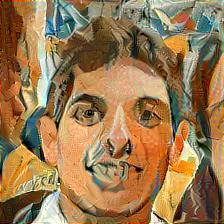
\includegraphics[width=0.98\textwidth]{../Images/transfer/tdf_demoiselles.jpg}
\end{minipage}
\caption{\textit{Gauche: Autoportrait au gilet vert de Delacroix - Droite: Les Demoiselles d'Avignon de Picasso}}
\label{fig:set_2}
\end{figure}

\paragraph*{Autoportrait au gilet vert - fig \ref{fig:set_2}} L'intérêt ici est qu'on transpose un portrait sur un visage donc on s'attend à ce que le visage ressorte mieux. C'est majoritairement le cas. L'algorithme se permet même de transposer avec quelques bémols le jeu de lumière dans les creux du visage de Delacroix vers mon visage. Mon pull bleu devient même verdâtre et mon manteau bleu prend la couleur de la redingote du peintre. Le visage en second plan est lui pour le coup très réussi car moins contrasté. Par contre la foule au fond est très mal rendue car le tableau ne possède pas de fond à part un ensemble marron teinté de rouge et de bleu qu'on voit apparaître dans le rendu de la foule. Il est à noter que l’œil droit est remarquablement bien rendu alors que le gauche moins (question d'illumination à mon avis). Le seul blanc sur le tableau provient de la chemise du peintre donc le rendu pour une zone spécifique comme les dents n'est pas très bon.

\paragraph*{Les Demoiselles d'Avignon - fig \ref{fig:set_2}} Picasso peint la chair et l'algorithme le comprend tout à fait et transpose à merveille les différentes teintes de peau sur le visage en respectant l'aspect cubique des personnages. Le nez prend aussi l'aspect deux points de vus en un. Les yeux sont bien rendus car il y a cinq exemples dans le tableau. L'algorithme comprend qu'il y a des personnages et un fond et décide donc de recréer ce fond en arrière-plan ce qui produit cet effet cohérent à l'arrière tout en respectant le fait qu'il y a un arbre qui n'appartient pas au même plan et qui est donc d'une couleur différente. Le personnage en second plan est mélangé avec l'arbre car ses cheveux peuvent déjà se "confondre" avec le tronc. Les dents posent encore problème avec un léger flou autour de la lèvre inférieure. Ce qui est étrange car c'est clairement dans le cubisme qu'on s'attend à trouver des formes pareilles ! 

\begin{figure}[!htb]
\centering
\begin{minipage}{0.25\textwidth}
\centering
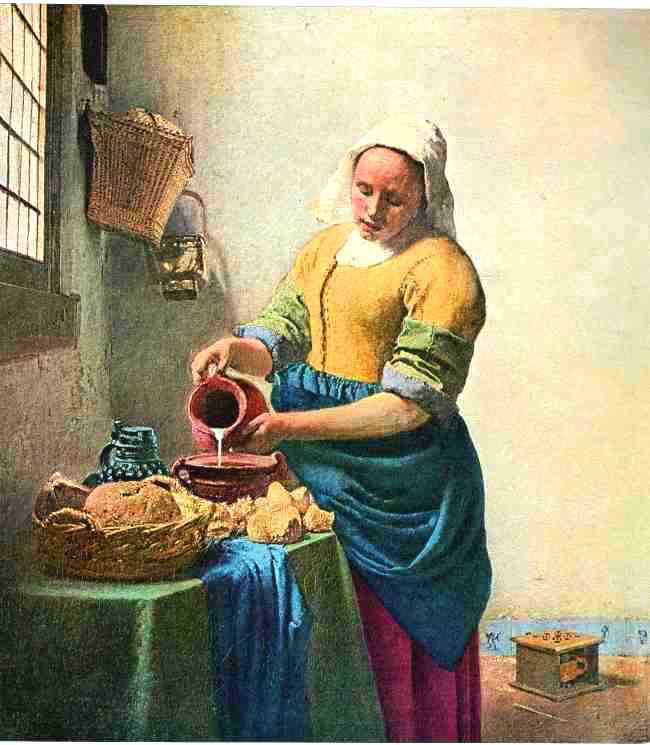
\includegraphics[width=0.98\textwidth]{../Images/laitiere.jpg}
\end{minipage}%
\begin{minipage}{0.25\textwidth}
\centering
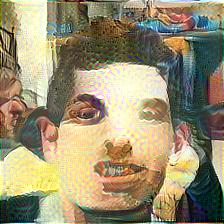
\includegraphics[width=0.98\textwidth]{../Images/transfer/tdf_laitiere.jpg}
\end{minipage}%
\begin{minipage}{0.25\textwidth}
\centering
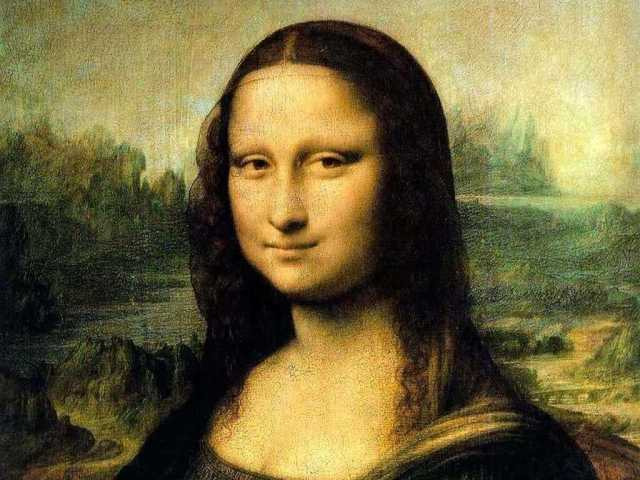
\includegraphics[width=0.98\textwidth]{../Images/joconde.jpg}
\end{minipage}%
\begin{minipage}{0.25\textwidth}
\centering
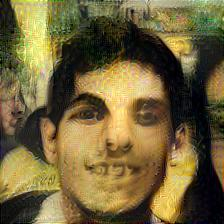
\includegraphics[width=0.98\textwidth]{../Images/transfer/tdf_joconde.jpg}
\end{minipage}
\caption{\textit{Gauche: La laitière de Vermeer - Droite: La Joconde de De Vinci}}
\label{fig:set_3}
\end{figure}

\paragraph*{La Laitière - fig \ref{fig:set_3}} Gros fiasco pour la Laitière de Vermeer en ce qui me concerne ! Le rendu du visage est très mauvais car la zone uniforme de la chair est prise pour le mur en arrière-plan. Par contre, très belle réussite pour la foule en arrière-plan qui est prise pour une table ! Le bout de tête de mon ami est fondu avec une nappe et on aperçoit un panier avec des fruits et des petits pots bleus carrés. Le réseau a donc appris le style d'une table façon Vermeer et reproduit la seule zone de détails là où il y en a. Les dents et les yeux font aussi apparaître des paniers ou des aliments ! enfin le tronc devient un mur  sur lequel y a un objet qui ressemble un peu à la fenêtre qu'on peut voir sur le tableau. Au-delà de reproduire le style du tableau, le réseau a recréé un décors proche de celui du tableau et ça, ce n'était pas gagné.

\paragraph*{La Joconde - fig \ref{fig:set_3}} Le résultat est à nouveau mitigé. Puisqu'on voit le visage de Monna Lisa, les yeux sont modifiés selon (mon regard ne vous suit pas comme celui de Monna). Le nez est par contre grotesquement élargis et le détail des dents est perdu à nouveau. L'arrière-plan possédant du contenu varié, l'algorithme choisit d'appliquer les teintes verdâtres des arbres plutôt que le ciel qui est choisi pour le tronc et les objets jaunes. Il est à noter aussi que les cheveux font apparaître des mèches sur le front et la tempe droite du visage à l'image des mèches de la Joconde. Encore une fois l'algorithme apprend le paterne des cheveux et l'applique à la photographie.

\begin{figure}[!htb]
\centering
\begin{minipage}{0.25\textwidth}
\centering
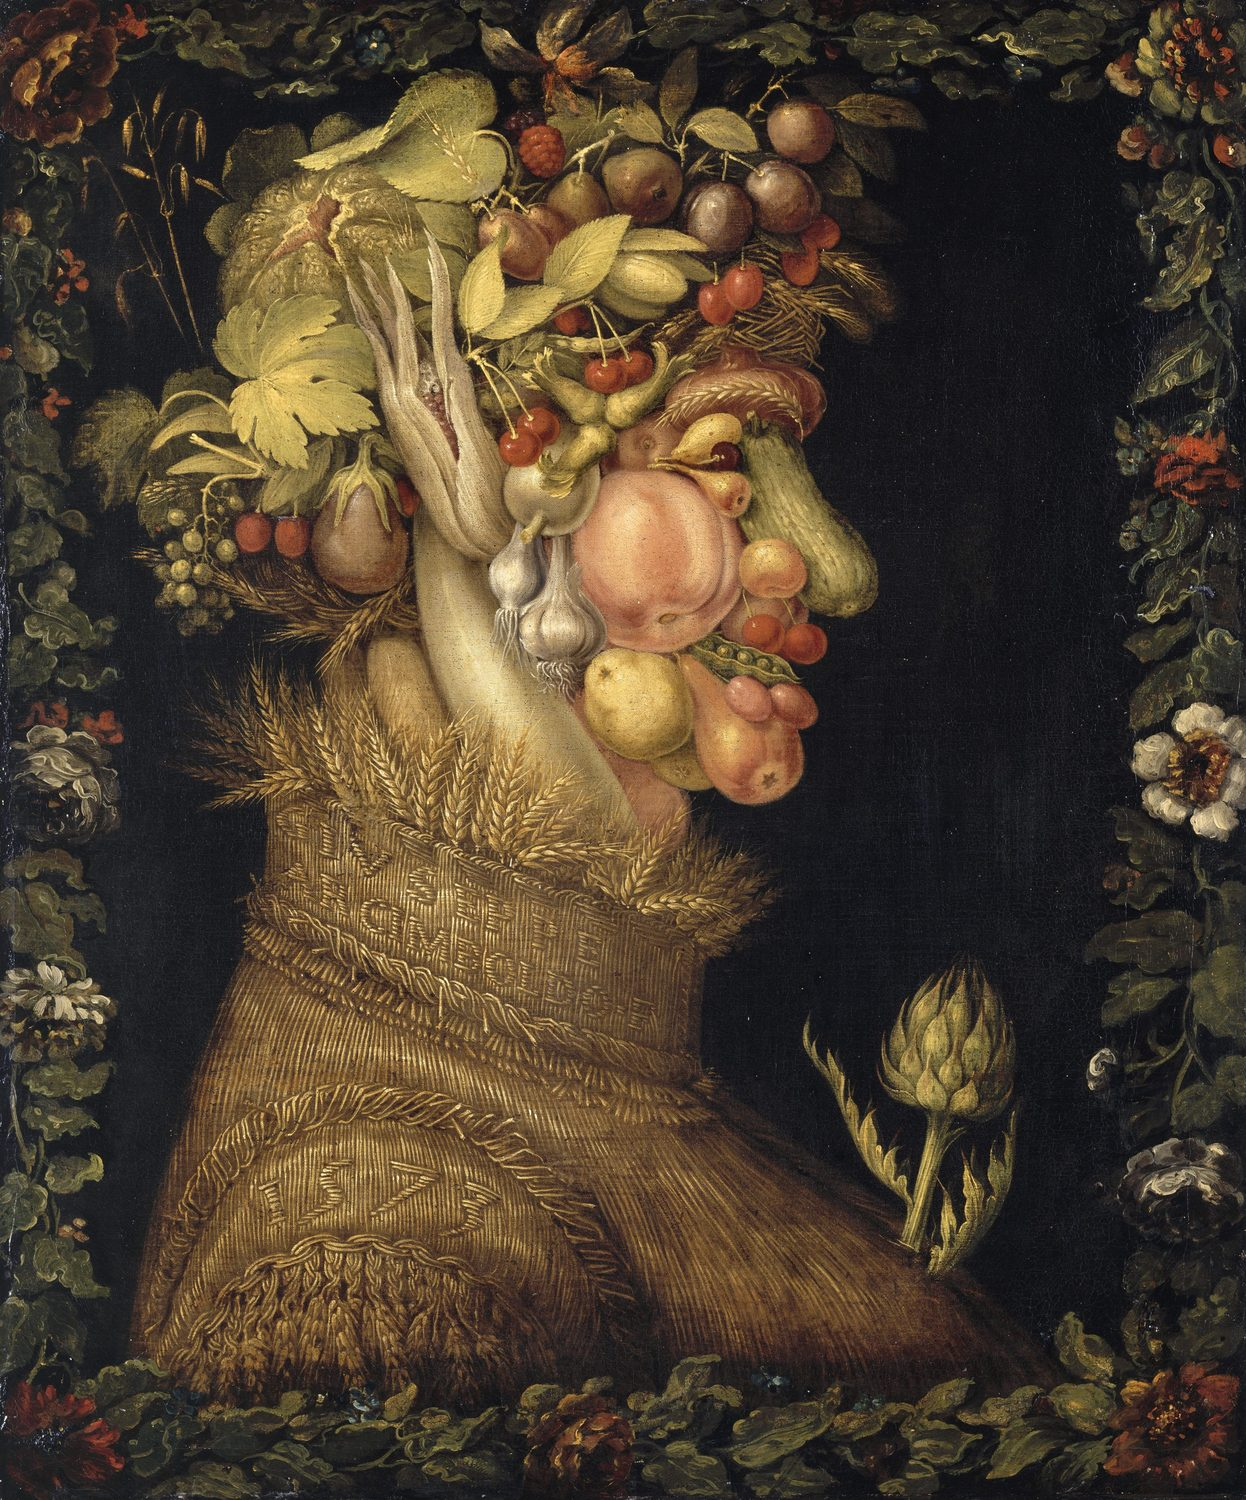
\includegraphics[width=0.98\textwidth]{../Images/arcimboldo.jpg}
\end{minipage}%
\begin{minipage}{0.25\textwidth}
\centering
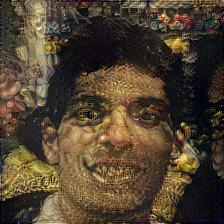
\includegraphics[width=0.98\textwidth]{../Images/transfer/tdf_arcimboldo.jpg}
\end{minipage}%
\begin{minipage}{0.25\textwidth}
\centering
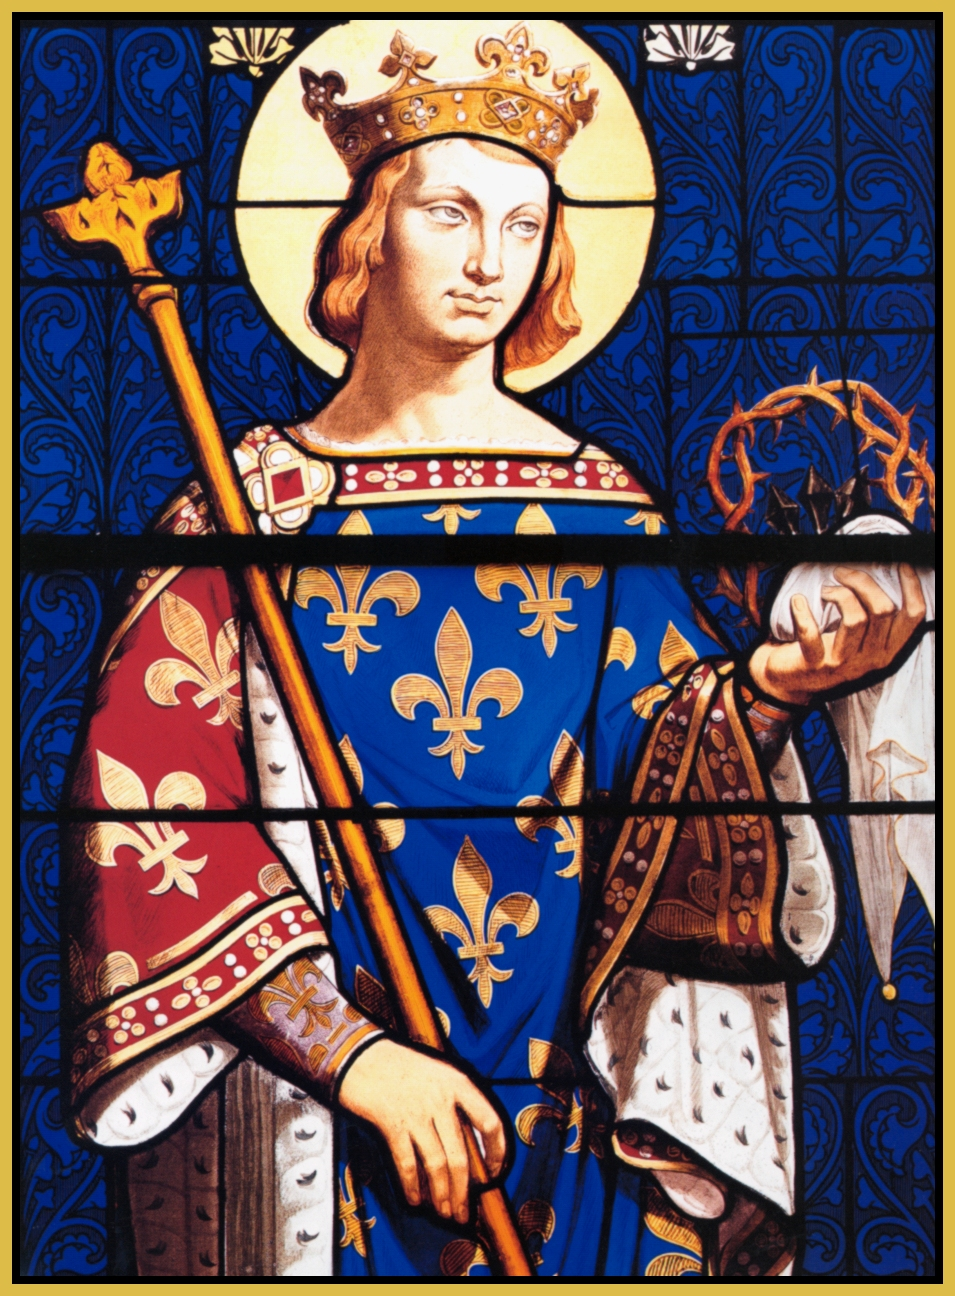
\includegraphics[width=0.98\textwidth]{../Images/vitraille.jpg}
\end{minipage}%
\begin{minipage}{0.25\textwidth}
\centering
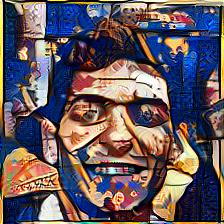
\includegraphics[width=0.98\textwidth]{../Images/transfer/tdf_vitraille.jpg}
\end{minipage}
\caption{\textit{Gauche:  Été d'Arcimboldo - Droite: Vitrail}}
\label{fig:set_4}
\end{figure}

\paragraph*{Été - fig \ref{fig:set_4}} Pour ce tableau d'Arcimboldo, l'aspect des fruits et légumes ne ressort pas sur mon visage qui est plutôt compris comme le manteau de blé du personnage sauf dans les zones de détails comme le nez. Le visage de mon ami et celui en second plan par contre possèdent chacun une texture plus proche de celle des fruits et des fleurs. Je pense que celui de mon ami fait apparaître des pétales car il est sur le bord comme là où se situent les plantes. L'arbre est complètement flouté et la foule en arrière-plan laisse difficilement percevoir des fruits et légumes de bonne résolution même sur les zones rouges ressemblent à des tomates ou des cerises.

\paragraph*{Vitrail - fig \ref{fig:set_4}} Voici un exemple présentant des lignes très bien définies et un découpage en rectangles. Le réseau interprète les changements de contraste comme des bordures de vitrail ce qui laisse apparaître ces bandes noires. De plus, il s'efforce à rendre la géométrie en rectangles et le fond bleu sur la rue. L'arbre est compris comme un pilier, le badaud en second plan est perdu la foule aussi. Les zones uniformes du visages produisent un effet patchwork car il n'y pas de grandes zones uniformes sur le vitrail. Les structures carrées comme les dents sont bien découpées mais la couleur est mauvaise et les yeux donnent aussi cet effet patchwork car la résolution des yeux de saint-Louis n'est pas assez bonne pour transposer les yeux comme dans le cas de Delacroix. Il est amusant de noter que comme pour Arcimboldo, le cadre doré est présent autour de l'image.

\begin{figure}[!htb]
\centering
\begin{minipage}{0.25\textwidth}
\centering
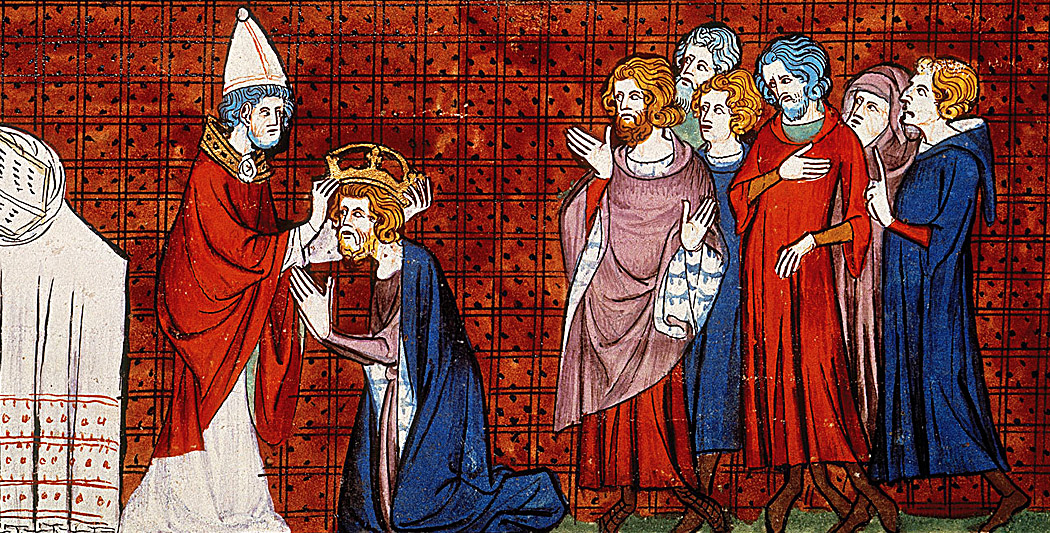
\includegraphics[width=0.98\textwidth]{../Images/charlemagne.jpg}
\end{minipage}%
\begin{minipage}{0.25\textwidth}
\centering
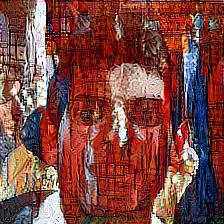
\includegraphics[width=0.98\textwidth]{../Images/transfer/tdf_charlemagne.jpg}
\end{minipage}%
\begin{minipage}{0.25\textwidth}
\centering
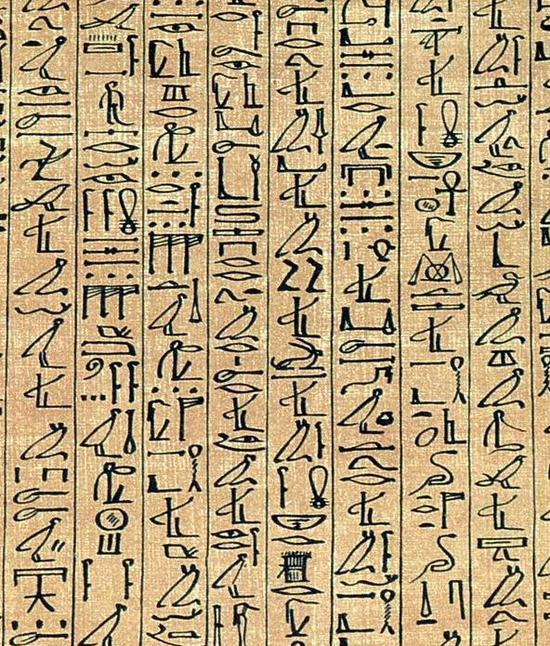
\includegraphics[width=0.98\textwidth]{../Images/papyrus.jpg}
\end{minipage}%
\begin{minipage}{0.25\textwidth}
\centering
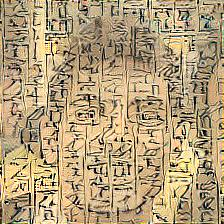
\includegraphics[width=0.98\textwidth]{../Images/transfer/tdf_papyrus.jpg}
\end{minipage}
\caption{\textit{Gauche: L'empereur Charlemagne - Droite: Morceau de papyrus}}
\label{fig:set_5}
\end{figure}

\paragraph*{Charlemagne - fig \ref{fig:set_5}} Comme dans le cas du vitrail, cette scène médiévale est représentée dans une image à l'aspect très géométrique et structuré. On ne voit pas bien les visages des protagonistes et le rouge est la couleur dominante avec quelques pointes de bleu. Le transfert se fait assez mal du coup et le rendu est très mauvais avec beaucoup de rouge pour représenter la chair, une autre teinte de rouge pour les cheveux bruns et encore un rouge tendant vers l'ocre en fond. L'arbre est blanc-gris car c'est la couleur la plus proche présente dans la scène. Je pense aussi que la position et la forme de l'autel joue beaucoup car l'autel peut être assimilé à l'arbre. C'est d'ailleurs pour cette raison qu'on perd le visage du badaud à mon avis. Les découpage en fonction du contraste et des zones détaillées comme les yeux et les dents sont bien respectées par contre grâce à la structure en maillage de l'image médiévale.

\paragraph*{Papyrus - fig \ref{fig:set_5}} On contenue dans les images à forte structure avec ce morceau de papyrus qui est un ensemble de colonnes avec des symboles. Comme dans \cite{DBLP:journals/corr/GatysEB15}, le réseau apprend à créer des symboles (ici des hiéroglyphes égyptiens), certes flous mais cohérents avec l'image de départ. De plus, on retrouve l'aspect colonne du parchemin mais les lignes suivent les contour de mon visage et du bout de visage de mon ami en donnant cet effet "cell-shading". Les zones détaillées laissent encore une fois apparaître des contours et des détails plus marqués grâce à la structure très géométrique de l'image de départ.

\begin{figure}
\centering
\begin{minipage}{0.25\textwidth}
\centering
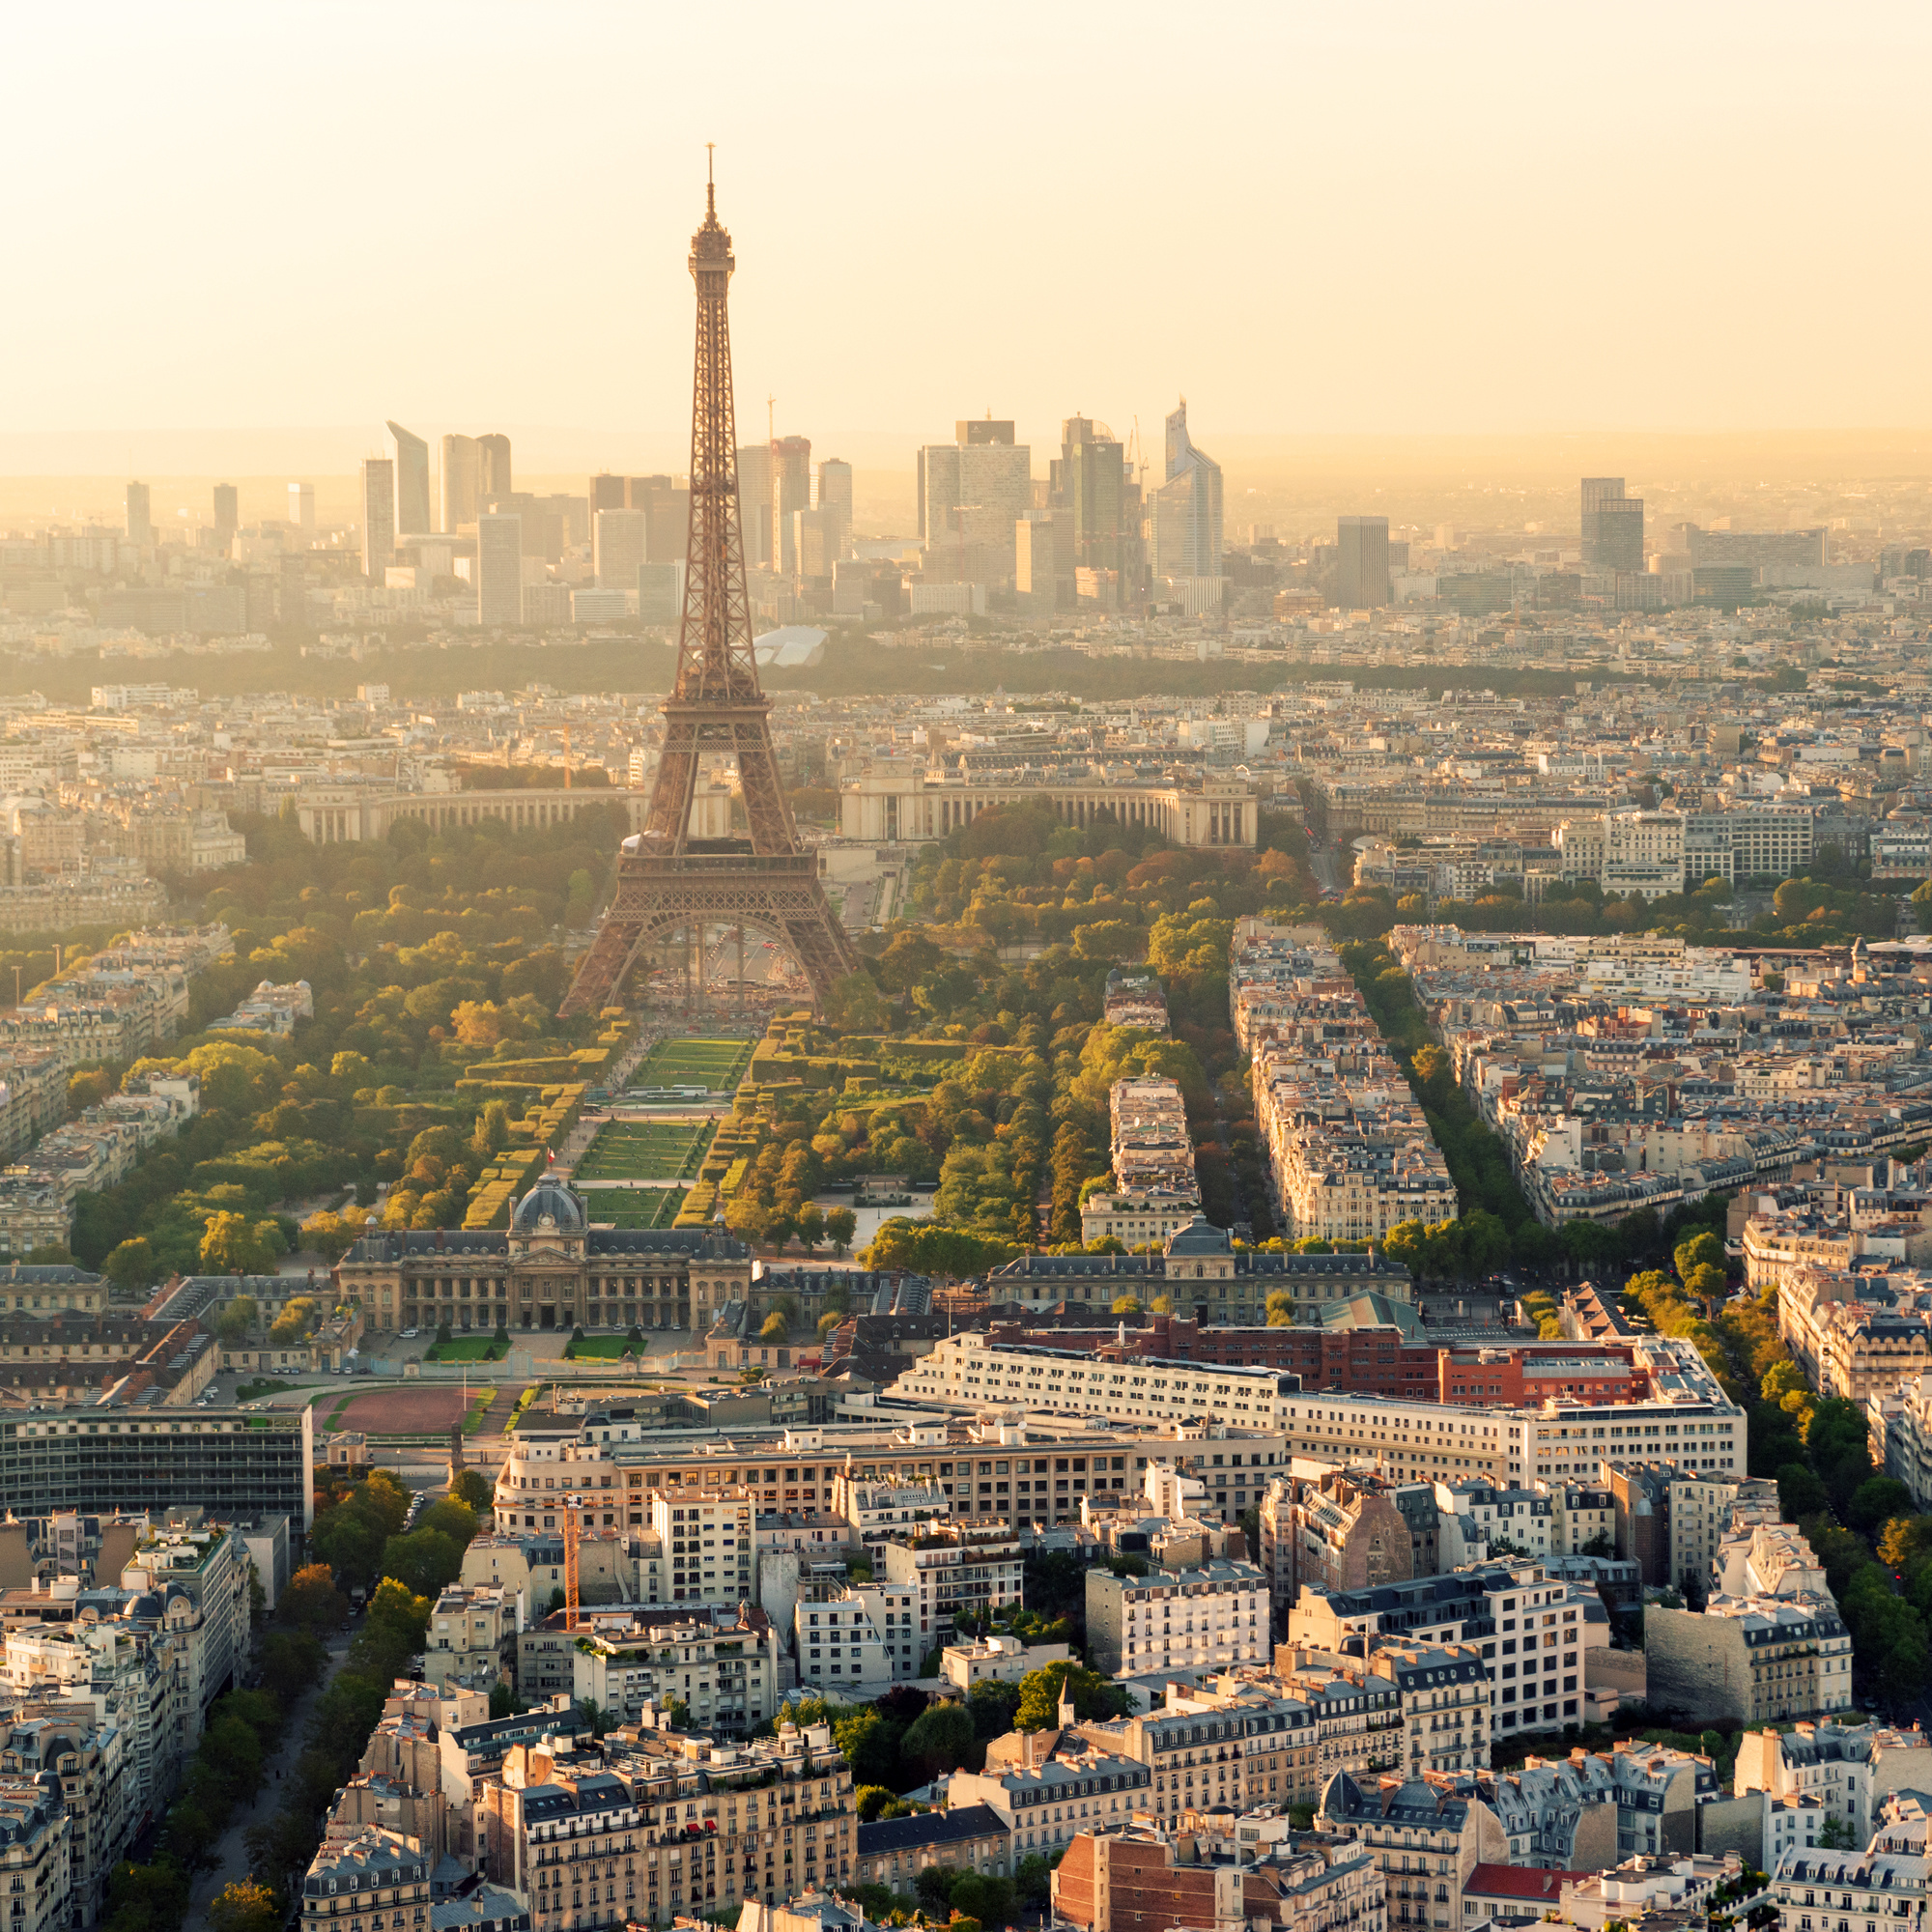
\includegraphics[width=0.98\textwidth]{../Images/paris.jpg}
\end{minipage}%
\begin{minipage}{0.25\textwidth}
\centering
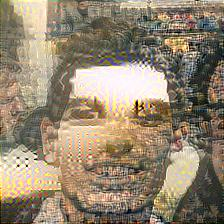
\includegraphics[width=0.98\textwidth]{../Images/transfer/tdf_paris.jpg}
\end{minipage}
\caption{\textit{Vue de Paris}}
\label{fig:set_6}
\end{figure}

\paragraph*{Photo de Paris - fig \ref{fig:set_6}} Pour clore cette série de transferts, je me suis demandé ce que pouvait produire le transfert de style d'une image naturelle vers une image naturelle; le résultat est très mauvais. La structure de l'image de départ est très bien reconnaissable car le style est le même ! On remarque quand même que ce qui marque particulièrement le réseau aussi, ce sont les fenêtres des immeubles en premier plan qui créent cet aspect mosaïque sur ma photo ! Mon visage étant une zone presque uniforme, le ciel y est transposé et mes yeux étant des zones de détails, on peut y voir des bouts de tour Eiffel.

\subsection*{Commentaires}
\paragraph*{} On remarque que le transfert de style ne se fait pas n'importe comment: les zones de mêmes couleurs et formes sont favorisées. Les géométries de l'image de style se retrouvent dans l'image générées ou alors s'adaptent à la structure de l'image de départ. Dans le cas échéant, le réseau applique le style du tableau et génère de l'information pour combler les différences comme pour l’Été d'Arcimboldo ou la Laitière de Vermeer ce qui est véritablement magique ! Ou pas.\\
On peut comprendre ces divers phénomènes en revenant à la structure même du réseau. Chaque couche applique des filtres capturant des informations différentes. Les filtres eux-mêmes possèdent des aspects différents comme le montrent les auteurs de \cite{DBLP:journals/corr/ZeilerF13}. Les premières couches prennent l'information sur les structures simples de l'image et ressemblent à des filtres DCT ou des ondelettes. Les couches plus hautes possèdent des filtres bizarres qui captent donc des informations plus en rapport avec les caractéristiques propres d'un objet. Le réseau produit donc des vecteurs de features dont certaines dimensions correspondent aux zones de basse-fréquences et d'autres aux zones de hautes fréquences et met en relation ces différentes features dimension par dimension lors du calcul de la perte. Je pense que si les informations dans les deux vecteurs dans une dimension sont proches (couleur, géométrie, etc), alors la descente de gradient trouve un compromis entre les deux images qui conserve beaucoup d'information de l'image de départ et modifie proportionnellement au ratio $\frac{\beta}{\alpha}$ l'information de départ. Dans le cas contraire, en fonction du même ratio, l'image de style écrase l'information de départ comme dans le cas de la Laitière en figure \ref{fig:set_3} où la foule étant un détail très différent des détails du tableau, le réseau préfère écraser la foule et mettre à la place une table avec des paniers.
 
\section*{Conclusion}
\paragraph*{}
Pour conclure, on a vu que le problème de transfert de style n'est qu'un problème d'optimisation sans contrainte. Au vu de la qualité des images dans la partie 3, on pourrait s'amuser à trouver des formes de régularisation pour améliorer le rendu de la génération et effacer ainsi certains artefacts (flou autour de la bouche pour le Picasso de la figure \ref{fig:set_2} par exemple). On pourrait se baser par exemple sur le modèle de \cite{DBLP:journals/corr/MahendranV14}.\\
La structure du réseau est au cœur de la qualité et de la quantité des éléments qui transitent d'une image vers une photographie et le fait que le calcul des distances inter-classes et intra-classes pour la classification se fassent de cette manière avec ces filtres en particulier permet donc de jouer sur le style et la structure et d'obtenir ainsi des vecteurs de features avec lesquels on peut jouer pour générer de nouvelles images. L'algorithme de rétro-propagation du gradient est l'autre clef de voûte de la solution au problème de transfert de style.\\
Ce rapport a donc permis tout au long de mettre en évidence les intérêts des différents paramètres dans le problème d'optimisation proposé dans la partie 2 puis le rôle joué par la génération de features dans la partie 3.


\section*{Sources des images originales}
\begin{enumerate}
\item Photo de Paris: www.tourmontparnasse56.com
\item Papyrus: www.isere.gouv.fr
\item Charlemagne: www.historyweb.fr
\item Vitrail de saint Louis: www.catholictradition.org/
\end{enumerate}

\bibliographystyle{plain}
\bibliography{biblio}



\end{document}